
\documentclass[11pt,letterpaper]{article}     % Tipo de documento y otras especificaciones
\usepackage[utf8]{inputenc}                   % Para escribir tildes y eñes
\usepackage[spanish]{babel}                   % Para que los títulos de figuras, tablas y otros estén en español
\addto\captionsspanish{\renewcommand{\tablename}{Tabla}}					% Cambiar nombre a tablas
\addto\captionsspanish{\renewcommand{\listtablename}{Índice de tablas}}		% Cambiar nombre a lista de tablas
\usepackage{geometry}                         
\geometry{left=30mm,right=30mm,top=25mm,bottom=28mm} % Tamaño del área de escritura de la página
\usepackage{ucs}
\usepackage{amsmath}      % Los paquetes ams son desarrollados por la American Mathematical Society
\usepackage{amsfonts}     % y mejoran la escritura de fórmulas y símbolos matemáticos.
\usepackage{amssymb}
\usepackage{graphicx}     % Para insertar gráficas
%\usepackage{graphics}     % Para insertar gráficas
\usepackage[lofdepth,lotdepth]{subfig}	% Para colocar varias figuras
\usepackage{unitsdef}	  % Para la presentación correcta de unidades
\usepackage{pdfpages}   %incluir paginas de pdf externo, para los anexos
\usepackage{appendix}   %para los anexos
\renewcommand{\unitvaluesep}{\hspace*{4pt}}	% Redimensionamiento del espacio entre magnitud y unidad
\usepackage[colorlinks=true,urlcolor=blue,linkcolor=black,citecolor=black]{hyperref}     % Para insertar hipervínculos y marcadores
\usepackage{float}		% Para ubicar las tablas y figuras justo después del texto
\usepackage{booktabs}	% Para hacer tablas más estilizadas

\usepackage{tikz} %preamble
\usepackage{pgfplots}
\usetikzlibrary{decorations.pathmorphing}
\usepackage{tikz-3dplot}
\usepackage{listings}
\lstset{language=C++}

\usepackage{cleveref}
\usepackage{hyperref}

\batchmode
%\usepackage{apacite}
\bibliographystyle{plain} 
\pagestyle{plain} 
\pagenumbering{arabic}
\usepackage{lastpage}
\usepackage{fancyhdr}	% Para manejar los encabezados y pies de página
\pagestyle{fancy}		% Contenido de los encabezados y pies de pagina
%%%%%%%%%%%%%%%%%%%%%%%%%%%%%%%%%%%%%%%%%%%%%%%%%%%%%%%%%%%%%%%%%%%%%%%%%%%%%%%%%%%%%%%%%%%%%%%%%%%%%%%%%%%%%%%%%%%%%%%%%%%%%%%%%%%%%%%%%%%%%%%%%
%No modificar las líneas anteriores


\lhead{Investigación bibliográfica II}
\chead{}
\rhead{IE-0217 - Estructuras abstractas.}	% Aquí va el numero de experimento, al igual que en el titulo
\lfoot{Escuela de Ingeniería Eléctrica}
\cfoot{\thepage\ de \pageref{LastPage}}
\rfoot{Universidad de Costa Rica}

\author{Autor: \\ \\Jean Carlos Chavarría Hughes, B11814\\ \\ \\ \\ \\Profesor:\\ \\Dr. rer. nat. Francisco Siles Canales \vspace*{2.0in}}
\title{Universidad de Costa Rica\\{\small Escuela de Ingeniería eléctrica\\ IE-0217 - Estructuras abstractas de datos y algor\' itmos para ingeniería\\II ciclo 2014\\\vspace*{0.55in} Investigación bibliográfica II}\\ Triangulac\' on geom\' etrica, con enf\' asis en el MoCap.
\vspace*{1.35in}}

%% Settings of tikz figures
\tikzset{isometricXYZ/.style={x={(-0.866cm,-0.5cm)}, y={(0.866cm,-0.5cm)}, z={(0cm,1cm)}}}
%: isometric South West : Z , South East : X , North : Y
\tikzset{isometricZXY/.style={x={(0.866cm,-0.5cm)}, y={(0cm,1cm)}, z={(-0.866cm,-0.5cm)}}}
%: isometric South West : Y , South East : Z , North : X
\tikzset{isometricYZX/.style={x={(0cm,1cm)}, y={(-0.866cm,-0.5cm)}, z={(0.866cm,-0.5cm)}}}


\begin{document}

\pdfbookmark[1]{Portada}{portada} 	% Marcador para el título

\maketitle
\newpage
\tableofcontents
\newpage
\listoffigures
\newpage

\section{Resumen}
En este proyecto se presentan una investigaci\' on bibliogr\' afica de la triangulaci\' on como t\' ecnica geom\' etrica para la determinaci\' on de posiciones de puntos, medidas de distancias o \' areas de figuras. As\' i como tambi\' en su implementaci\' on en las t\' ecnicas de MoCaps \' opticos con m\' as de una c\' amara, como por ejemplo el OptiTrack.

\section{T\' itulo}
El uso de la triangulaci\' on en el MoCap.

\section{Problema Principal}
El desconomiento interno de los m\' etodos internos que se implementan en dispositivos tecnol\' ogicos, como por ejemplo el OptiTrack generalmente no tiene consecuencias que lamentar. Sin embargo cuando se refiere a usos de investigaci\' on acad\' emica, resulta crucial conocer a fondo como se realizan todos los m\' etodos para lograr explotar al m\' aximo sus capacidades y obtener el m\' aximo desempe\~ no posible.

\section{Justificación}
Con esta investigaci\' on se busca resolver el problema que existe en la actualidad dentro de la Escuela de Ingenier\' ia El\' ectrica relacionado con el desconocimiento del funcionamiento interno de ciertos equipos tecnol\' ogicos, espec\' ificamente brindar una descripci\' on breve y precisa del c\' omo se implementa la triangulaci\' on en el OptiTrack que se encuentra dentro del Laboratorio de Investigaci\' on: PRISLAB.

\section{Metodolog\' ia}
La presente investigaci\' on es de car\' acter bibliogr\' afico que se centra en la recolecci\' on principal de informaci\' on en libros, art\' iculos y la p\' agina virtual principal del OptiTrack.

\section{Objetivos}
\subsection{Objetivo General}
Presentar una base te\' orica comprensible sobre la t\' ecnica geom\' etrica de la triangulaci\' on espacial, con \' enfasis en su implementaci\' on dentro del MoCap.
\subsection{Objetivos Espec\' ificos} 
%Recuerde que se realiza un capitulo de investigacion por cada objetivo especifico. Sin perder de vista el objetivo general.
\begin{enumerate}
\item Pormenorizar de manera minuciosa la t\' ecnica  de triangulaci\' on trigonom\' etrica.

\item Comprender el uso de la triangulaci\' on en el MoCap.
\begin{itemize}
\item Estudiar los fundamentos de la geometr\' ia epipolar.
\end{itemize}
\end{enumerate}

\section{Introducci\' on}

El m\' etodo de la triangulaci\' on de ha utilizado desde la antiguidad para medir distancias y posiciones por los antiguos egipcios y debido a su gran capacidad, la t\' ecnica fue evolucionando a trav\' es de los a\~ nos hasta llegar a las t\' ecnicas modernas de redes de triangulaci\' on que se utilizan en la actualidad, como por ejemplo los sistemas de posicionamiento global, GPS.

Se puede hablar de que los grades investigadores y pioneras del tema son: Snell, Tales, Pei Xiu, Liu Hui y Picard.
En lo que concierne a la t\' ecnica del \textbf{Motion Capture}, lo que se hace en t\' erminos generales es implementar marcadores especiales como reflectores de luz que envien de regreso un rayo de luz hacia la c\' amara, y mediante el proceso de la triangulaci\' on con varias c\' amaras, la posici\' on de los marcadores se almacenan en puntos (X,Y,Z), tal como se puede observar en la Figura \ref{fig:usoMOCAP}.

Por otra parte, la geometr\' ia epipolar es un surgimiento de la necesirar del estudio de visi\' on est\' erea en su total generalidad, mediante t\' ecnicas de c\' alculo avanzada y el uso de la matriz fundamental y la matriz escencial.

\begin{figure}[hbtp]
\caption{Uso del MOCAP de la Escuela}
\centering
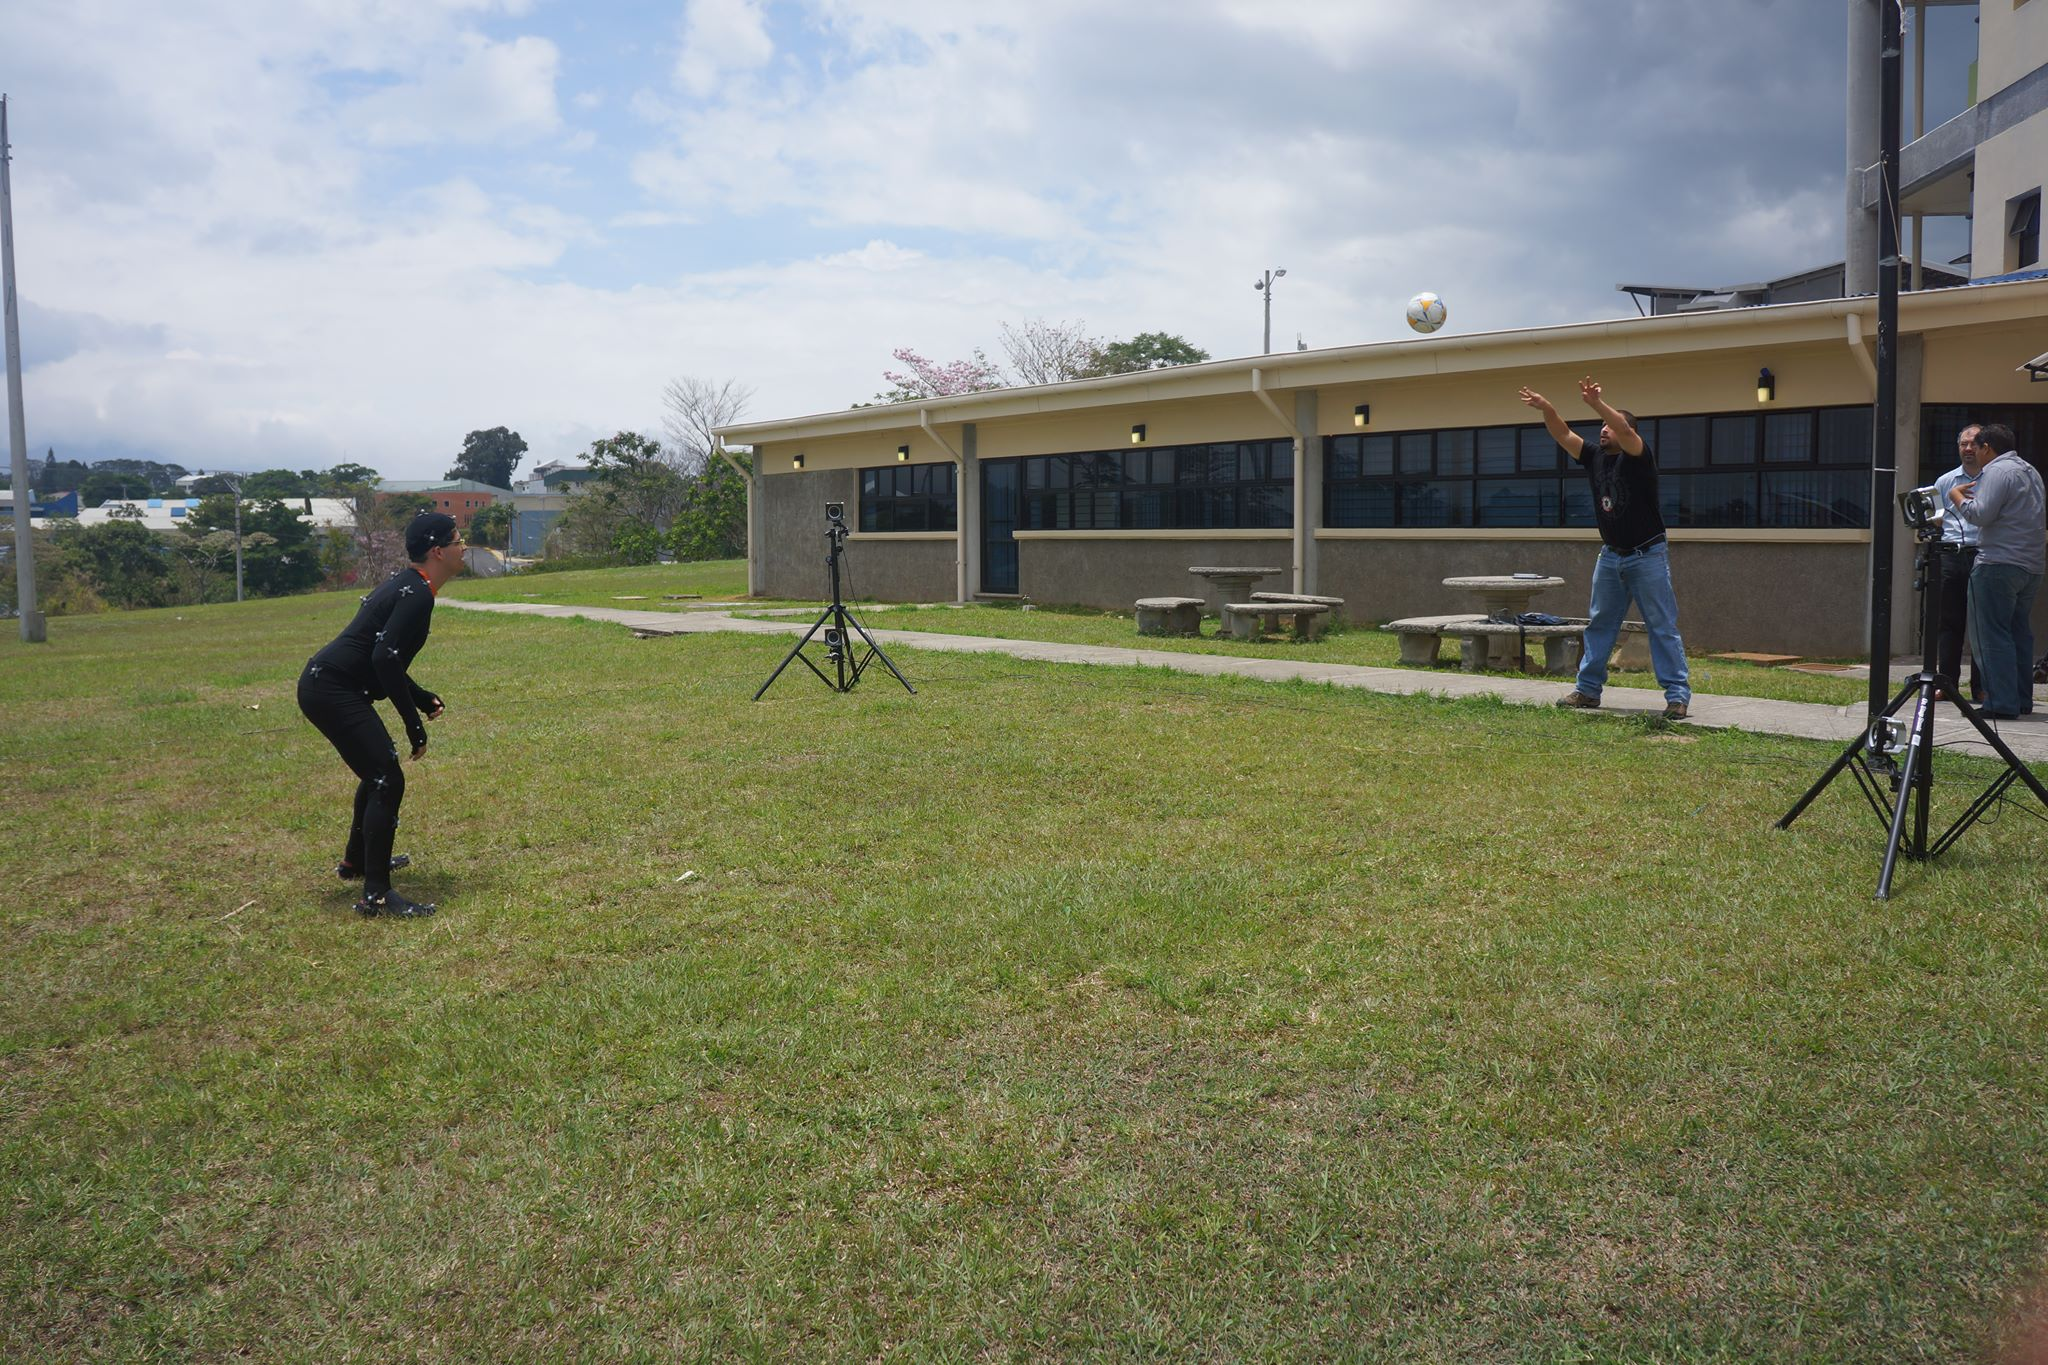
\includegraphics[scale=0.25]{imagenes/1614262_755232877844886_6375624551639752710_o.jpg}
\label{fig:usoMOCAP}
\end{figure}



\section{Desarrollo}
%%Capitulo 1
\subsection{Capitulo 1:Pormenorizaci \'on de la triangulaci\' on trigonom\' etrica}
La resolución de triángulos es un ejercicio matemático de infinidad de aplicaciones prácticas. Una de estas aplicaciones, quizá la más usada en distintos ámbitos es el cálculo de distancias que, de manera directa, serían imposibles de medir por problemas de situación, de entorno. 
En t\' erminos generales, la t\' ecnica consiste en completar triángulos de manera que sean resolubles, es decir, que se conozcan los elementos suficientes como para calcular los demás, y aplicar los teoremas de seno o del coseno y la definición de las razones trigonométricas para hacer el resto. 

Este m\' etodo se remonta desde los a\~ nos 1625, con el cient\' ifico Giovanni Cassini, en Italia. El mismo fue capaz de utilizar por primer vez los conceptos desarrollados por Galileo, relacionados con mediciones trianguladas.

La demostraci\' on formal, se basa en la geometr\' ia Euclideana y la ley de senos y cosenos se puede observar en el documento:  \url{http://scimath.unl.edu/MIM/files/MATExamFiles/Sehnert_FinalMEXP_LA_WS.pdf}
 pero el enfoque de este documento pretende dar una explicaci\' on menos formal del m\' etodo por lo que se omite su demostraci\' on. 
 
 Se puede entender f\'  acilmente con el ejemplo de la Figura \ref{fig:ejemplo1}, donde se tiene un punto B, del cual se desconoce su ubicaci\' on en el espacio, pero se cuenta tres dispositivos que son capaces de determinar la distancia entre tal dispositivo y el punto B. As\' i, se forman tres circunferencias conc\' entricas en cada dispositivo, y de radio igual a la distancia entre dicho dispositivo y el punto B. Entonces la intersecci\' on de las tres circunferencias es la posici\' on del punto B en el espacio.

\begin{figure}[hbtp]
\caption{Ejemplo de triangulaci\' on}
\centering
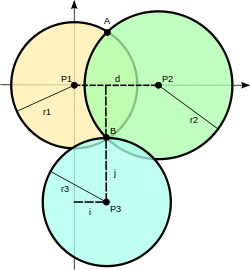
\includegraphics[scale=1]{imagenes/250px-Trilateration.png}
\label{fig:ejemplo1}
\end{figure}

\url{http://upload.wikimedia.org/wikipedia/commons/7/7e/Trilateraci%C3%B3n.svg}

 

%%Capitulo 2
\subsection{Capitulo 2: Uso de la triangulaci\' on en el MoCap.}

Las c\' amaras de captura de movimiento son colocadas alrededor del volumen en perspectivas diferentes, luego la herramienta de calibraci \' on se coloca y mueve alrededor del volumen. Esto da informaci\' on necesaria al software para determinar donde esta cada c\' amara en el volumen. Cuando m\' ultiples c\' amaras son usadas en diferentes perspectivas, y el sofware conoce la posici\' on de cada una a trav\' es de la calibraci\' on, entonces es capaz de \textbf{ver} el viaje de los puntos desde diferentes \' angulos y triangular la localizaci\' on tridimensional en el volumen. Este proceso es similar en todas las t\' ecticas volum\' etricas de mocaps, en las cuales se necesite determinar posiciones tridimensionales, tal como se observa en la Figura \ref{fig:4camaras}


\begin{figure}[hbtp]
\caption{Set de captura de video}
\centering
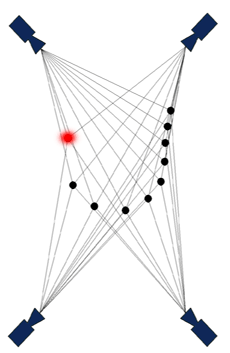
\includegraphics[scale=1]{imagenes/ppt_area.png}
\label{fig:4camaras}
\end{figure}


La obtenci\' on de esta informaci\' on no es trivial, de hecho se lleva a cabo mediante el seguimiento óptico, la cual utiliza una señal de emisión de luz o marcadores pasivos a detectar a la persona u objeto. Con el marcador, el movimiento de las imágenes capturadas  se puede calcular por triangulación, as\' i como tambi\' en la posición de los marcadores en 3D. 
Métodos estereoscópicas a menudo hacen que sea más fácil de detectar la localizaci\' on del objeto, ya que el objeto puede ser detectado a partir de la triangulación de con la posición de la cámara.

Adem\' as, se menciona que aunque la t\' ecnica solo puede ser implementada por dos c\' amaras, se necesitan tres y esto es debido a que si en un momento de que se deba determinar la interseccion entre dos lineas, otro marcados esta estorbando, entonces se use una tercer camara para evitar el problema.

En t\' erminos generales, dentro del proceso de seguimiento de marcadores hasta la implementaci\' on del modelo abstracto, se siguen una serie de pasos por parte del MoCap, los cuales se pueden emnumerar como:

\textbf{Rastreo}.
\begin{enumerate} 
\item De puntos 2D a trazos 2D.
\item Uni\' on de trazos 2D con el l\' imite epipolar para crear trazos en 3D.
\item Condensado de trazos 3D.
\item Uni\' on de trazos 3D.
\end{enumerate}

\textbf{Rectificaci\' on}.
\begin{enumerate} 
\item Clasificaci\' on de trazos de acuerdo a los marcadores.
\item Estimaci\' on del modelo 3D.
\end{enumerate}

Se puede considerar que la triangulaci\' on se implementa en el primer paso de la primera parte, pero luego se habla de un l\' imite epipolar, el cual ser\' a analizado en la siguiente secc\' on.




%Motion Capture
%Triangulation
%Introduction

%Optical Motion Capture works on the simple principle of inverse projection and triangulation. The complexities (especially in systems like Vicon) come extensions of these basic principles, but in general the basic idea is still the same.

%Inverse Projection

%Inverse Projection takes the inverse route followed by perspective projection in 3D graphics (whereby a 3D scene is presented as a 2D image using a view frustum and the loss of z-depth). In this case, we have a 2D image and we need to determine the 3D space that the camera is viewing. As with perspective projection we need to have knowledge of the frustum (along with a few other correctional elements), in this way we are basically assigning a line from a pixel on the 2D image as being a line from that pixel back through the lens and into the 3D space (we can see this as a side view in Figure 1a).

%Triangulation

%Therefore, anything that intersects that line will be represented in that pixel, so in general we have an idea of where in space along the X, Y coordinate system of the camera's 3D space the object the pixel is representing is; but we do not know anything about the Z-position (because we don't have that information). The only thing we do know about the Z-direction is that if we can see it on the 2D image, it must not be occluded.

%In order to determine the Z-position of that object's position, we need to use another camera (which is obviously not in the same position as the original camera). In this case, we follow the same procedure for the second camera and determine which pixel produces a line that intersects our original line. If we know the position of the two cameras (even only relatively) then we can use this information to determine the Z-position of the object.

%The Third Camera

%In general, having 2 cameras should be sufficient for triangulation, however we are essentially determining the position of a marker from the intersection of two lines; problems occur when a another marker is occluding that intersection. In this case the two rays from the original two cameras will intersect, but it will create a false intersection. In this case a 3rd camera can help validate the position of an intersection (as it will not be occluded by the same marker).


\section{Capitulo 3: Implementaci\' on de la geometr\' ia epipolar.}

El l\' imite epipolar es un elemento de la geometr\' ia epipolar, la cual se le llama al tipo de geometr\' ia que se encarga de caracterizar la visi\' on est\' ereo. Por ejemplo cuando 2 c\' amaras ven una escena en 3D desde dos distintas posiciones (como sucede naturalemente en el mundo real).

El nombre de geometr\' ia epipolar es debido a que los puntos en los cuales la recta que une los centros de proyecci\' on de las c\' amaras corta a los planos de proyecci\' on se llaman epipolos. De esta manera se puede hablar de punto epipolar, l\' inea epipolar, plano epipolar, l\' imite epipolar y triangulaci\' on epipolar.


La importancia práctica de la geometr\' ia epipolar arranca del hecho que el plano identificado por P, O
i, Od, el llamado plano epipolar, interseca cada imagen en una l\' inea llamada l\' inea epipolar. Consideremos el triple P, pi y pd. Dado pi, P puede caer en cualquier punto del rayo definido por Oi y pi.
Pero dado que la imagen de este rayo en la imagen derecha es la l\' inea epipolar a trav\' es del punto correspondiente pd dicho punto debe estar sobre la l\' inea epipolar. Esta correspondencia establece una aplicaci\' on entre puntos de la imagen izquierda y rectas de la imagen derecha y viceversa. Una consecuencia de esta
correspondencia es, que dado que todos los rayos pasan por construcci\' on por el centro de proyecci\' on, todas las rectas epipolares deben pasar por el epipolo.
Por tanto si determinamos la aplicaci\' on entre puntos de la imagen izquierda(derecha) y las rectas epipolares de la imagen derecha(izquierda), podemos restringir la b\' usqueda para el emparejamiento de pi a lo largo de la
l\' inea epipolar correspondiente. As\' i pues la b\' usqueda de las correspondencias se reduce a un problema 1D.
Alternativamente este conocimiento tambi\' en se puede usar para verificar s\' i una potencial pareja de puntos correspondientes, lo son de verdad o no. Esta t\' ecnica es normalmente una de las m\' es efectivas para detectar las posibles falsas correspondencias debidas a oclusi\' on, tal y como se observa en la Figura \ref{fig:epipolar}.

\begin{figure}[hbtp]
\caption{Principio del plano epipolar}
\centering
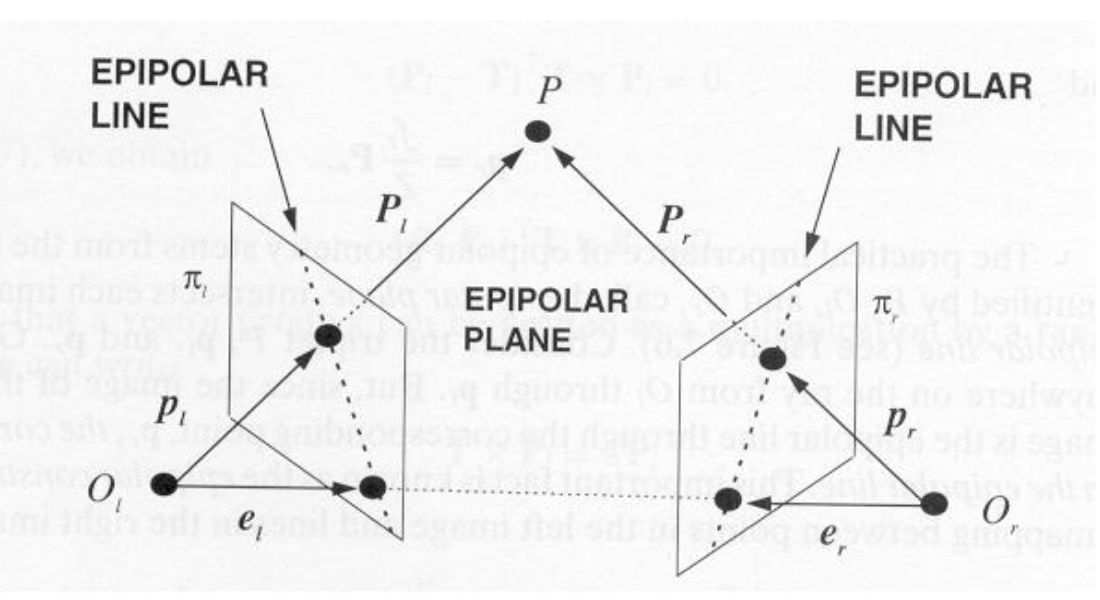
\includegraphics[scale=0.21]{imagenes/planoEpipolar.png}
\label{fig:epipolar}
\end{figure}


\section{Conclusiones}
\begin{figure}[hbtp]
\caption{Imlementaci\' on del NAO}
\centering
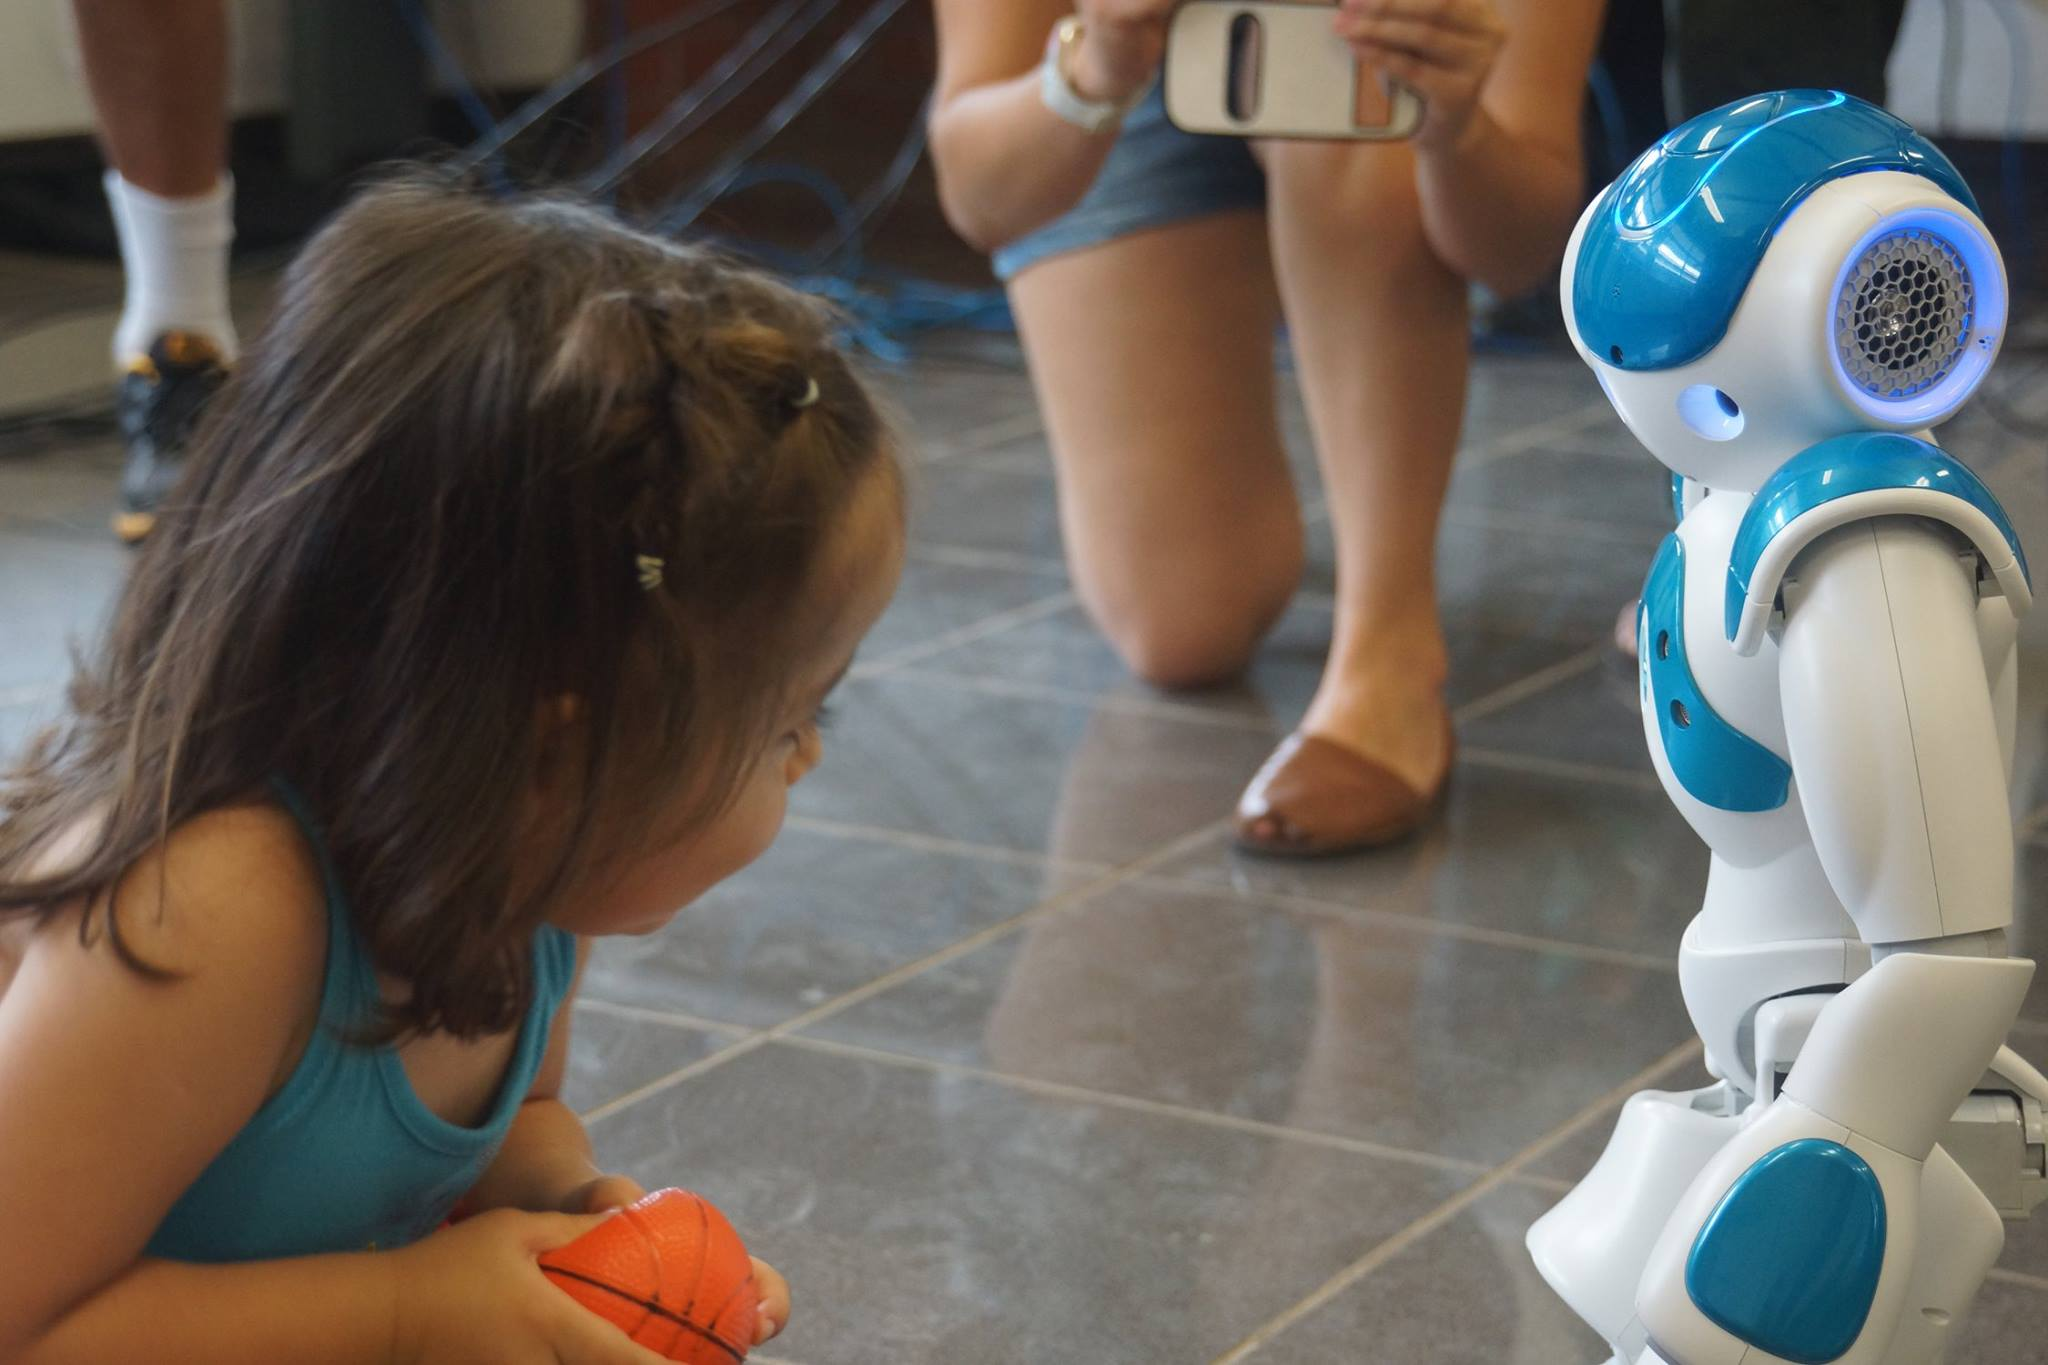
\includegraphics[scale=0.15]{imagenes/10553806_792493910785449_7200970304906961642_o.jpg}
\end{figure}




\newpage
\renewcommand{\bibname}{Referencias}
\addcontentsline{toc}{section}{Referencias}

\begin{thebibliography}{5}
\bibitem {3D Motion Reconstruction} Mingyu Chen, Ghassan AlRegib, and Biing-Hwang Juang, (2011). \textit{Trajectory triangulation: 3D motion reconstruction with $l1$ optimization}. School of electrical and computer engineering, Georgia Institute of Technology.


\bibitem {Vicon MX System} Motion Capture, Carleton Unersity, Ottawa, Ontario, Canada..  \textit{Vicon MX system} Recuperado de \url{http://mocap.csit.carleton.ca/index.php?Section=Overview&Item=MotionCapture&Page=Triangulation} el 7 de octubre de 2014.

\bibitem {Optical Motion Standford} Optical Motion Capture Guide. \textit{A Guide to Optical Capture} Obtenido de \url{http://physbam.stanford.edu/cs448x/old/Optical_Motion_Capture_Guide.html}  el 7 de octubre de 2014.


\bibitem {SpotLight} SpotLight on Multimedia. \textit{Spotlight} Obtenido de \url{http://www.spotlight-multimedia.com/tutorials/animation/74-motion-capture.html}  el 7 de octubre de 2014.

\bibitem {JorgeFernandez} Calculo de distancias por triangulaci\' on. \textit{Triangulacion} Obtenido de \url{http://www.jorge-fernandez.es/proyectos/angulo/temas/temapc/index.html}  el 14 de octubre de 2014.

\bibitem {Giovanni Cassini} Triangulaci\' on, demostraci\' on formal \textit{Triangulaci\' on} Obtenido de \url{http://scimath.unl.edu/MIM/files/MATExamFiles/Sehnert_FinalMEXP_LA_WS.pdf}  el 14 de octubre de 2014.

\bibitem {Magazine} Post Magazine: Motion Capture \textit{Motion Capture Magazine} Obtenido de \url{http://www.postmagazine.com/Publications/Post-Magazine/2008/May-1-2008/MOTION-CAPTURE.aspx} el 14 de octubre de 2014.



\end{thebibliography} 
\end{document}